\section{Construction}\label{sec:construction}

Before diving into the details of the pseudocode, we give an intuitive overview
of the \rollerblade construction.

% TODO: Consider whether there is duplication with the introduction here

There are $m$ \rollerblade clients numbered $1, 2, \ldots, j, \ldots, m$
and $n$ underlying protocols $\Y[][1], \Y[][2], \ldots, \Y[][i], \ldots, \Y[][n]$.
Each $\RB[j]$ of the clients runs a full node for each of the $n$ underlying
ledger protocols,
$\Y[j][1], \Y[j][2], \ldots, \Y[j][i], \ldots, \Y[j][n]$.
Each $\RB[j]$ \emph{simulates} within its implementation $n$ different instances
of the overlay protocol $\Pi$,
$\Z[j][1], \Z[j][2], \ldots, \Z[j][i], \ldots, \Z[j][n]$,
one for every underlying ledger protocol,
$\Y[j][1], \Y[j][2], \ldots, \Y[j][i], \ldots, \Y[j][n]$.
% TODO: figure

The \rollerblade client $\RB[j]$ allows the external user to issue a \emph{write} instruction
with some \data
to any $i^\text{th}$ simulated machine $\Z[j][i]$. This is done as follows. When the user
of $\RB[j]$ issues a \emph{write} instruction to $\Z[j][i]$, this instruction is not given to
$\Z[j][i]$ directly. Instead, it is serialized into a string and \emph{encoded} into a transaction
to be recorded on the respective underlying ledger $\Y[j][i]$. This is captured by
the \writeToMachine function illustrated in Algorithm~\ref{alg.read-write}.
The encoding functionality is made available because
the underlying ledgers are assumed to be bulletin boards.
When the `write' instruction becomes recorded in the ledger $\Ledger[j][i]$ reported
by $\Y[j][i]$, then it will be passed to the simulated
machine $\Z[j][i]$ as soon as the respective round simulation takes place.
Through this recording of machine inputs on-ledger, we intent for other
rollerblade clients $\RB[j']$ to replicate the exact simulation of $\Z[j'][i]$ for that
same $i$ (in the Analysis section, this is made precise in Conjecture~\ref{conj:cross-party}).
Additionally, the external user can, at any time, issue a \emph{read} instruction to
the simulated machine $\Z[j][i]$, without affecting its current state (recall that we
require $\Pi$'s \emph{read} method to not alter the machine's internal state upon completion).

Each of $\Z[j][i]$ is simulated in a per-round basis by having its \emph{execute}
function invoked once per round $r$. When it is simulated, it expects its \emph{write} function to have
been called some ($0$ or more) number of times prior to \emph{execute} being invoked,
indicating user input for round $r$. When \emph{execute} is invoked, it has access to read
and write into the network through the authenticated channels interface $\net$.
When it \emph{reads} from the network, it consumes network messages that other machines
have dispersed into the network during previous rounds (potentially with some delay $\Delta$).

In order to simulate this communication between machines, the system works as follows.
A \emph{relayer} node is tasked with \emph{checkpointing} every ledger to every other ledger
during every round. There is no trust placed upon this relayer, but at least one relayer
is assumed to be honest (a client can run its own relayer if it so wishes, so this does
not introduce any additional trust assumptions). Checkpointing is performed as follows.
The relayer runs a full node in each of the underlying protocols $\Y[][i]$ and
invokes the \emph{transcribe} function $\Y[][i].\transcribe()$ to obtain a transcription
$\tau$; this functionality is made available because underlying ledgers are assumed to be
transcribable. This transcription is then checkpointed into every other ledger protocol
$\Y[][i']$ by \emph{encoding} it into a bulletin transaction $\tx = \Y[][i'].\encode(\tau)$
and \emph{writing} it into $\Y[][i']$. The relayer is illustrated in
Algorithm~\ref{alg.relayer}.

\emph{These ``write'' and ``checkpoint'' instructions are the only thing ever written
to the ledger from the honest rollerblade clients}. In particular, no network outputs
produced by any of the $\Z[j][i]$ are ever written on the ledger. Instead, we observe
that reading the checkpoints is sufficient for each rollerblade client to reproduce
the network outputs of all simulated machines.

Let us now explore, in more detail, how this simulation works. Each rollerblade execution
of a particular overlay protocol $\Pi$ on top of a certain number of underlying ledger
protocols $\Y$ is marked with a \emph{session id} \sid in order to achieve context
separation with other rollerblades running, potentially different, protocols $\Pi'$
on top of a, potentially different but not disjoint, set of underlying ledger protocols
$\Y[][']$. This \sid is placed into every instruction recorded on-ledger, in particular
the `write' and `checkpoint' instructions.

The simulation only runs
on-demand when the user of $\RB[j]$ issues a \emph{read} instruction to the machine
$\Z[j][i]$. The user can indicate that the read instruction pertains to a particular
round $\simulationRound$, and the \emph{read} instruction is conveyed to the snapshot
of $\Z[j][i]$ immediate after round $\simulationRound$ has been executed.

The entry point for $\RB[j]$'s reading from a simulated machine
is illustrated in Algorithm~\ref{alg.read-write}.
The \readFromMachine function takes the \sid, the overlay protocol $\Pi$ to run,
the identity $i$ of the simulated machine to read from,
and the array of underlying ledger protocol instances $\Y[j]$
(corresponding to the full node parties maintained by $\RB[j]$),
with $|\Y[j]| = n$. Additionally, the round for which the read is requested
is passed in the \simulationRound parameter, and \realityRound denotes the
current round of the external clock of $\RB[j]$. During our analysis, we will
see that, while \simulationRound and \realityRound pass at the same rate,
the user of $\RB[j]$ must wait for some \realityRound rounds for the simulation
to ``settle'' before he can invoke \readFromMachine with the respective \simulationRound.
The \readFromMachine machine function simulates the execution of the machine
$\Z[j][i]$ using the data obtained by \emph{reading} the ledger $\Ledger[j][i]$
reported by $\Y[j][i]$ at round \realityRound. Upon reading the ledger,
the \readFromMachine function invokes the \simulate function to obtain an instance
of the $\Z[j][i]$ machine executed up to round \simulationRound (inclusive).
Lastly, the \readFromMachine function invokes the \lread function of the simulated
machine $\Z[j][i]$ right after the \simulationRound execution has completed.

The core simulation is implemented in the function \simulate illustrated in
Algorithm~\ref{alg.simulate}, which takes parameters with the same semantics as
the \readFromMachine function parameters. The job of the \simulate function
is to simulate the execution of machine $\Z[j][i]$ up to, and including, round
$\simulationRound$. This is all done within the mind of machine $\RB[j]$,
with no external communication at all. Upon completing the simulation,
the \simulate function returns the instance of the machine $\Z[j][i]$,
which can be used to apply \lread on it by the user.

Additionally, the
\simulate function returns all the network outputs that $\Z[j][i]$
produced during the simulation, which we call its \emph{outboxes}
(Line~\ref{alg.simulate:return}). The outboxes (initialized in
Line~\ref{alg.simulate:outboxes-init}) are structured as an array
containing one \emph{outbox} per index, each index corresponding to
a round of execution. In particular $\outboxes[r]$ contains the
outbox produced by simulated party $\Z[j][i]$ during round $r$.
This outbox $\outboxes[r]$, produced during round $r$, is a list
of authenticated messages \netouts. Each such authenticated
message \netout in \netouts is a dictionary containing two entries:
The \emph{to} entry is a number between $1$ and $n$
indicating the recipient of the message; the \emph{msg}
entry is the string of the message to be delivered.
Since rounds begin at $0$, the entry $\outboxes[0]$ is the
empty outbox (ensured in its initialization in
Line~\ref{alg.simulate:outboxes-init}).

To conduct the simulation, the \simulate function initially calls
\prepareSimulationInputs (Line~\ref{alg.simulate:recursion}),
which prepares two arrays \emph{writeboxes}
and \emph{inboxes} to be used by the simulation of $\Z[j][i]$.
These sequences are produced by reading the ledger $\Ledger[j][i]$.
\emph{The whole simulation of $\Z[j][i]$ is based only on the data
recorded on its respective ledger.}
The array \emph{writeboxes} is structured as an array containing
one \emph{writebox} per index, each index corresponding to a
round of execution. In particular, $\writeboxes[r]$ contains the
writebox to be used prior to the execution of round $r$.
The writebox $\writeboxes[r]$ is a list of strings each of which must be
written using the \emph{write} functionality of $\Z[j][i]$
before \emph{execute} is invoked for round $r$.
These writes correspond to (honestly or adversarially) recorded
`write' instructions on the ledger $\Ledger[j][i]$.
The data structure $\inboxes$ is structured similarly.
The inbox $\inboxes[r]$ contains the inbox to be used \emph{during}
the execution of $\Z[j][i]$ at round $r$. The inbox $\inboxes[r]$
is a list of authenticated messages \netins. Each such authenticated
message \netin in \netins is a dictionary containing two entries:
The \emph{from} entry is a number between $1$ and $n$ indicating the
sender of the message; the \emph{msg} entry is the string of
the message to be delivered.

The simulation begins by initializing a new machine $\Z[j][i]$
from scratch (Line~\ref{alg.simulate:construct}). The simulation
proceeds in rounds managed by the main loop in
Line~\ref{alg.simulate:for}. For each iteration of this \emph{for}
loop, the \emph{execute} function of the simulated machine
is invoked, once per every round $r$. In preparation of the
execution for round $r$, we have to invoke the \emph{write}
function of $\Z[j][i]$ for every write in the writebox pertaining
to round $r$. This is performed in the \emph{for} loop of
Line~\ref{alg.simulate:write}, which invokes $\Z[j][i]$'s
\emph{write} method for each \emph{write} in the current
round's writebox.

During initialization (Line~\ref{alg.simulate:construct}),
the simulated machine is
initialized by giving it access to the network oracle $\net$.
Whereas, normally, the protocol $\Pi$ would have expected this
oracle to realize an authenticated channels functionality, we
\emph{trap} the calls to the network \emph{send} and network
\emph{receive} functions that the instance $\Z[j][i]$ of $\Pi$
may call and we replace them with our own implementation based on
the underlying ledgers. The trapped functions are implemented
in Line~\ref{alg.simulate:send} and Line~\ref{alg.simulate:receive}
respectively. The machine $\Z[j][i]$ may invoke the network
\emph{send} method, during its \emph{execute} invocation, zero
or more times during the round. When the network \emph{send} method
is invoked by $\Z[j][i]$, the message is \emph{not} conveyed
to other machines. Instead, it is appended to the array
$\outboxThisRound$. The variable contains the append-only
outbox produced by the simulation during round $r$. It is
initialized as the empty array
(Line~\ref{alg.simulate:outboxThisRound-init}) at the beginning
of every round. Upon the completion of a round's execution,
the particular outbox is appended to the list of all outboxes
(Line~\ref{alg.simulate:outboxes-append}).
Lastly, in preparation for the execution of round $r$,
the variable $\inboxThisRound$ is initialized to
$\inboxes[r - 1]$ (Line~\ref{alg.simulate:netin})
and is an inbox containing the network messages to be
delivered at round $r$ (and may have been disbursed during
rounds $r - \Delta, \ldots, r - 1$). This inbox is returned
whenever the simulated machine calls the network \emph{receive}
function of the oracle \net. The variable \inboxThisRound
is reassigned at the beginning of every round.

Once the last iteration of the \emph{for} loop of Line~\ref{alg.simulate:for} completes,
the simulated machine $\Z[j][i]$ has concluded its execution of rounds $1, \ldots, \simulationRound$.
At the end of the simulation, the \simulate function returns the \outboxes generated by
$\Z[j][i]$ throughout its execution as well as the machine instance $\Z[j][i]$ itself.
The machine instance can be used for example to call \emph{read} on it.

The last piece of the puzzle is the \prepareSimulationInputs function which is
called by \simulate. This function receives as input the ledger $\Ledger[j][i]$ and
returns the \writeboxes and \inboxes to be used by \simulate to simulate the machine $\Z[j][i]$. It will be important for
our security results that the output of \prepareSimulationInputs is deterministic
and depends only on the ledger $\Ledger[j][i]$ and not on any of the other ledgers $\Ledger[j][i'], i' \neq i$.

In particular, the function \prepareSimulationInputs receives as parameters the \sid of the \rollerblade, the
overlay protocol $\Pi$, the underlying index $i$, the ledger $\Ledger[j][i]$, all the underlying ledger protocol instances $\Y[j]$,
the simulation round \simulationRound, and the round \realityRound during which the ledger $\Ledger[j][i]$ was read.
The method begins by initializing \inboxes and \writeboxes. For every round $r = 0 \ldots \simulationRound$ we set
$\inboxes[r]$ and $\writeboxes[r]$ to be empty lists initially (Line~\ref{alg.prepare-simulation-inputs:init}). The entries $\inboxes[0]$ and $\writeboxes[0]$ will remain empty
since the simulation begins at round $1$ with an empty \inbox and \writebox.

The rest of the indices in $\inboxes$
and $\writeboxes$ we fill in by reading the relevant rollerblade transactions within $\Ledger[j][i]$. Initially, the relevant transactions are extracted from the ledger $\Ledger[j][i]$ into a sequence of instructions $L$ by invoking $\decodeUnderlying$ (Line~\ref{alg.prepare-simulation-inptus:decode-underlying}). The sequence $L$ contains pairs $(r, \instruction)$ of instructions, each accompanied by the round with which the relevant instruction was recorded on the ledger $\Ledger[j][i]$. This is where we will use the temporal nature of the underlying ledger $\Ledger[j][i]$: The round $r$ recorded on-ledger for the instruction $\instruction$ is the round of the simulation of $\Z[j][i]$ in which we will utilize this instruction.

The instructions in $L$ are processed sequentially by the \emph{for} loop in Line~\ref{alg.prepare-simulation-inputs:for}. As we are only interested in the data necessary to simulate up to round $\simulationRound$, we can conclude this loop early if we see a transaction recorded with round $r \geq \simulationRound$ (Line~\ref{alg.prepare-simulation-inputs:early-exit}). The easy case is when the instruction type is a `write'. In that case, we extend the writebox $\writeboxes[r]$ for round $r$ by appending the data $\instruction.\data$ to be written to it (Line~\ref{alg.prepare-simulation-inputs:write}).

The more complicated case pertains to instruction type `checkpoint'. This is a checkpoint from underlying ledger $i'$ to underlying ledger $i$, i.e., concerns a certificate of ledger $i'$ that was recorded onto ledger $i$. This certificate's data $\instruction.\data.\certificate$ is fully recorded within $\Ledger[j][i]$ and does not require reading from $\Y[j][i']$. The function $\untranscribe$ of $\Y[j][i']$ is used to untranscribe this certificate into a ledger $\ImaginaryLedger[j][i']$ (Line~\ref{alg.prepare-simulation-inputs:untranscribe}), but the return value of this untranscribe function does not at all depend on the local state of $\Y[j][i']$, but only on the parameter $\instruction.\data.\certificate$ passed to it. This ``imaginary ledger'' $\ImaginaryLedger[j][i']$ extracted from untranscribing is the ledger with index $i'$ extracted based on the data included within $i$. It is possible that $\ImaginaryLedger[j][i'] \neq \Y[j][i'].\lread()$ (especially if ledger $i'$ is unsafe).

This ledger $\ImaginaryLedger[j][i']$, obtained by untranscribing, is then passed into a \emph{new} \simulate invocation for machine $\Z[j][i']$ (Line~\ref{alg.prepare-simulation-inputs:recursion}). This simulation is performed based on ledger $\ImaginaryLedger[j][i']$ and not on $\Y[j][i'].\lread()$, and so may differ from the result of invoking \simulate using $\Ledger[j][i'] = \Y[j][i'].\lread()$. The \simulate function is executed up to simulation round $r - u_i - v_{i'} - 1$ (the reason for this arithmetic will become apparent in the security proof). The \emph{outboxes} returned from this simulation of ledger $i'$ are then collected and translated into inboxes for consumption by the simulation of ledger $i$ (Line~\ref{alg.prepare-simulation-inputs:outboxes-to-input})

This

% \subsection{A Majority Vote}\label{sec:construction-naive}
%
% Composing many underlying ledgers into an overlay ledger is not complicated, but it is complex
% protocol, with many moving parts. As such, we present the design in iterative stages. In the
% first stage, presented in the present section, we provide a design based on an \emph{honest majority}
% approach. This obvious approach introduces the notation and allows us to familiarize the reader
% with the concepts, but is ultimately misguided. However, it is imperative for understanding why
% a straightforward solution is not applicable, and a stepping stone for the next development in
% the protocol. In the section that follows, we introduce a BFT layer running on top of our
% underlying ledgers. This is our final construction, but we describe it intuitively first before
% we delve into the technical details of a precisely defined construction in the next section.
% We leave the formal analysis and proofs of security for the end.
%
% The first and obvious approach to compose ledgers starts by the assumption that the
% underlying majority is secure. The core idea is to produce the overlay ledger by taking
% a majority vote on the reported underlying ledgers. The construction is illustrated in
% Figure~\ref{fig.naive}, where
% $m$ parties $\RB[1], \ldots, \RB[m]$ run the overlay protocol.
% Each of the $\RB$ nodes runs
% a full node to each of the $n$ underlying DLPs $\wheel[1], \ldots, \wheel[n]$, pictured as squares
% of varying shades of yellow. The full nodes communicate with one another using their
% respective DLP technology, which we treat as a black box here, depicted as elongated
% rectangles in varying shades of red towards the bottom of the figure.
% The $\RB$ nodes
% make their own overlay DLP, offering \emph{read} and \emph{write} functionalities.
%
% \begin{figure*}
%     \centering
%     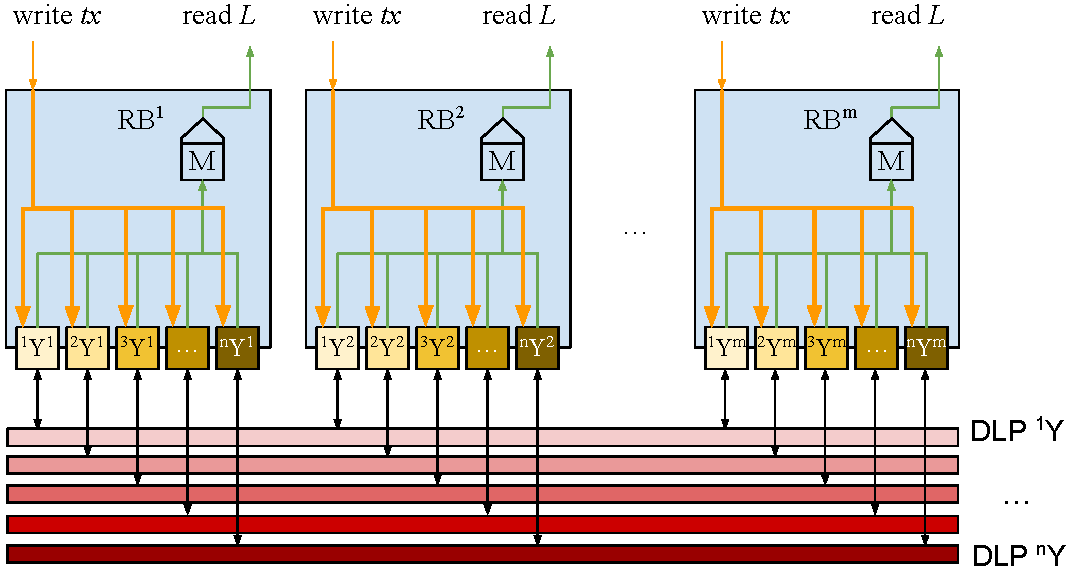
\includegraphics[width=\textwidth,keepaspectratio]{figures/rollerblade-naive-construction.pdf}
%     \caption{The first attempt at the composed construction. Here,
%              $m$ different parties $\RB_1, \ldots, \RB_m$ operate Rollerblade
%              nodes, each of which runs a client on $n$ different underlying
%              DLPs $Y_1, \ldots, Y_n$.}
%     \label{fig.naive}
% \end{figure*}
%
% When an $\RB$ transaction $\tx$ is \emph{written} into one of the $\RB$ nodes by the user,
% the $\RB$ serializes this transaction for each of the underlying DLPs (using the
% serialization mechanism particular to each individual DLP) and posts it
% as a transaction there, depicted as orange wires running downwards in the figure.
% Let us walk through
% this process precisely.
% The $\RB$ party takes $\tx$ and wraps it in a \emph{message}
% which is the pair $m = (`\text{write}', \tx)$.
% This captures the user intent to \emph{write} this overlay transaction to the underlying ledgers.
% The first element of the pair (\emph{`write'}) indicates the \emph{type} of message.
% As we evolve our protocol, we will introduce other control message types later, but,
% for now, this is our only message type. Once the message is created, we pass it to
% \textsf{encodeRollerbladeTx}, listed in Algorithm~\ref{alg.encode}.
% This function first serializes $m$
% into a string $s = \textsf{serialize}(m)$. This string is then encoded for each particular
% underlying DLP $\wheel[i]$ by invoking the bulletin functionality $\wheel[i]\text{.encode}$.
% This returns a transaction $\tx'_j$, which is appropriate for being written to $\wheel[i]$.
% Note that $\tx$ is a transaction of the overlay ledger, whereas each of $\tx'_i$ is a
% transaction of the underlying ledger $\wheel[i]$. Each resulting underlying transaction $\tx'_i$
% is then broadcast into $\wheel[i][j]$ by having $\RB[j]$ invoke the \emph{write}
% functionality of $\wheel[i][j]$.
%
% \import{./}{algorithms/alg-encode}
%
% Each transaction $\tx'_i$ is written to the respective underlying DLP $\wheel[i][j]$ during
% the same round $r$. If $i$ happens to be live, the respective \emph{read} call of all
% other $j'$ DLPs on $\wheel[i][j']$ at round $r' \geq r + u$ will result in a ledger
% $\wheel[i][j'][r']$ containing $\tx'_i$.
%
% In order to answer a particular overlay \emph{read} call, the overlay party $\RB[j']$ must
% issue a \emph{read} to all of its underlying DLPs $\wheel[1][j'], \ldots, \wheel[n][j']$,
% depicted as green wires running upwards in the figure.
% The transactions in $\wheel[i][j'][r']$ are of $\wheel[i]$ format,
% and therefore must be decoded using the bulletin decoding functionality
% appropriate to each underlying DLP $\wheel[i]$.
% Those that decode successfully result in a string $s$ which can, in turn,
% be deserialized into a message $m = (`write', \tx)$ containing the type \emph{`write'}
% and the overlay transaction $\tx$. The process of decoding and deserializing a transaction
% is done through the \textsf{decodeRollerbladeTx} algorithm, listed in Algorithm~\ref{alg.encode}.
% It invokes \textsf{decodeRollerbladeTx} in each of the returned ledgers, resulting
% in a sequence of $n$ ledgers $\overline{L}$, each a sequence of overlay transactions.
% We call this process \emph{sanitization} and list it in Algorithm~\ref{alg.sanitize}.
%%
% Next, the overlay party $\RB[j']$ will need a mechanism to combine these sanitized ledgers
% into \emph{one} ledger in order to answer the \emph{read} call from the user.
% The sanitized ledgers are fed into a \emph{majority voting} contraption, denoted with
% the letter M and the \emph{house} symbol in the figure, which then outputs the desired
% ledger $L$ of $\RB$ transactions (top).
% The idea is that, if the majority of underlying ledgers is secure, the transaction $\tx$
% in question will eventually appear (liveness) and stabilize (safety) in a majority of them.
% The party $\RB[j']$ can therefore take a majority vote among the underlying ledgers
% to extract an overlay ledger aspiring to be safe and live.
% The algorithm listed in Algorithm~\ref{alg.majorityvote} performs the majority voting
% process. It is invoked when the user of $\RB[j]$ invokes \emph{read} at a certain
% round $r$. The process accepts a list of ledgers $\overline{L}$ each $\prescript{i}{}{\overline{L}}$
% of which contains the sanitization of the underlying ledger $\wheel[i][j][r]$.
% The majority of $\overline{L}$ will contain all the honest
% transactions issued at least $u$ rounds ago. It goes through each
% position in the sanitized ledgers. For each position $k \in \mathbb{N}$,
% it observes what each of the $n$ ledgers report in the $k^\text{th}$ position.
% The reported transactions in the $k^\text{th}$ position are
% $\wheel[1][j][r][k], \wheel[2][j][r][k], \ldots, \wheel[n][j][r][k]$.
% The algorithm counts the frequency of appearance of each transaction at
% the position $k$. If a transaction
% appears more than $\frac{n}{2}$ times in this position, it is included in the sanitized ledger
% (since we have $n$ underlying ledgers, only one transaction can do so).
% Otherwise, if no transaction appears more than $\frac{n}{2}$, the sanitized ledger
% is cut short and returned.
%
% \import{./}{algorithms/alg-majorityvote}
%
% The intuition why this majority voting \emph{should work} is this: An honest
% transaction will eventually be included in all of the underlying ledgers that
% are live, and hence will appear in more than $\frac{n}{2}$ underlying ledgers
% and will make it to the output of \textsf{MajorityVote}. Since the majority
% of underlying ledgers is secure, they will maintain the transaction order,
% and so will the output of \textsf{MajorityVote}. In order for the adversary
% to censor a transaction from the final ledger, the adversary will need to
% break the security of more than $\frac{n}{2}$ underlying ledgers.
%
% Unfortunately, this argument does not hold water. The reason is that, due to
% delays, two transactions $\tx_1$ and $\tx_2$ may appear in a different order
% in different underlying ledgers, even if all of them are secure. It is possible
% that $\tx_1$ appears before $\tx_2$ in $\lfloor \frac{n}{2} \rfloor$ of the
% underlying ledgers, whereas it appears after $\tx_2$ in the $\lceil \frac{n}{2} \rceil$
% of the rest\footnote{In fact, it is possible, even with every underlying ledger being
% secure, that each ledger reports a particular order of transactions, but the majority voting
% cannot not result in an order at all. This is known as a Condorcet cycle~\cite{condorcet}.}.
% The adversary can then easily swap the transaction order by
% breaking the security of only one chain. Therefore, this initial design
% is not secure. We are now ready to rectify this issue by introducing a more
% nuanced mechanism in place of majority voting.
%
% \subsection{A BFT to Rule Them All}\label{sec:construction-bft}
%
% \begin{itemize}
%   \item Simple majority voting construction with no BFT protocol on top. Serialization and deserialization requirements and algorithms. Majority voting on ``ledger extensions'' algorithm. Fragile results in which different blockchains can disagree on the order and one blockchain can ``flip over'' the result. l. Condorcet cycles.
%   \item The necessity of running a BFT protocol on top, but without talking about the oracle abstraction of signatures, broadcasting, verification, and receiving. Light clients from one blockchain to another using smart contracts. Using the blockchains as ports of communication.
%   \item Oraclizing sign/broadcast and receive/verify.
%   \item Remove the smart contract assumption using dirty ledgers.
%   \item The full construction.
% \end{itemize}
%
% \subsection{Compatibility}\label{sec:compatibility}
%

\import{./}{algorithms/alg-relay}
\import{./}{algorithms/alg-decode-underlying}
\import{./}{algorithms/alg-outboxes-to-inbox}
\import{./}{algorithms/alg-prepare-simulation-inputs}
\import{./}{algorithms/alg-simulate}
\import{./}{algorithms/alg-read-write}

%
% \section{New material 2023-04-19}
%
% Known origin oracle.
%
% \import{./}{algorithms/alg-known-origin}
% \import{./}{algorithms/alg-transferable-origin}
%
% \dionyziz{TODO: recursive transferable origin oracle; gossip oracle}
%
% A distributed protocol amendable to the \rollerblade transform must be given as
% an oraclized \emph{deterministic} Turing Machine designed to work with the
% $\fko$ or $\fto$ functionalities as an oracle.
%
% \begin{enumerate}
%   \item Table of analogies: $u$-liveness = $\Delta$-delay; GST = eventual liveness; safety failure = RR failure; party = ledger...
%   \item Rollerblade ledger: A construction of a ledger protocol on top of rollerblade.
% \end{enumerate}
%
% % TODO: Remark: Dolev--Strong can be ran on top of \rollerblade. This is useful when combined with interoperability.
%
